% TU Delft Beamer template
% Author: Maarten Abbink
% Delft University of Technology
% March 2014
% Version 2.0
% Based on original version 1.0 of Carl Schneider
\documentclass{beamer}
\usepackage[english]{babel}
\usepackage{calc}
\usepackage[absolute,overlay]{textpos}
\usepackage{animate}
\usepackage{amssymb,amsmath}
\usepackage{booktabs}
\usepackage{textcomp}
\usepackage{graphicx}
\usepackage{multimedia}
\usepackage{subcaption} 
\usepackage{multirow}
\newcommand{\tabitem}{~~\llap{\textbullet}~~}


\mode<presentation>{\usetheme{tud}}

\title[Triogen Turbine Optimization]{Triogen Turbine Optimization}
%\subtitle[Effects of height ratio and rotational]{Effects of height ratio and rotational speed}
\subtitle[Analysis]{Euler turbine model analysis}
\institute[TU Delft]{Delft University of Technology}
\author{Stephan Smit}
\date{\today}

% Insert frame before each subsection (requires 2 latex runs)
\AtBeginSubsection[] {
	\begin{frame}<beamer>\frametitle{\titleSubsec}
		\tableofcontents[currentsection,currentsubsection]  % Generation of the Table of Contents
	\end{frame}
}
% Define the title of each inserted pre-subsection frame
\newcommand*\titleSubsec{Next Subsection}
% Define the title of the "Table of Contents" frame
\newcommand*\titleTOC{Outline}

% define a symbol which can be removed if you don't need it
\newcommand{\field}[1]{\mathbb{#1}}
\newcommand{\Zset}{\field{Z}}
\newcommand{\resfdir}{../results/figures/}
\newcommand{\resmdir}{../results/movies/}
\begin{document}

{
% remove the next line if you don't want a background image
\usebackgroundtemplate{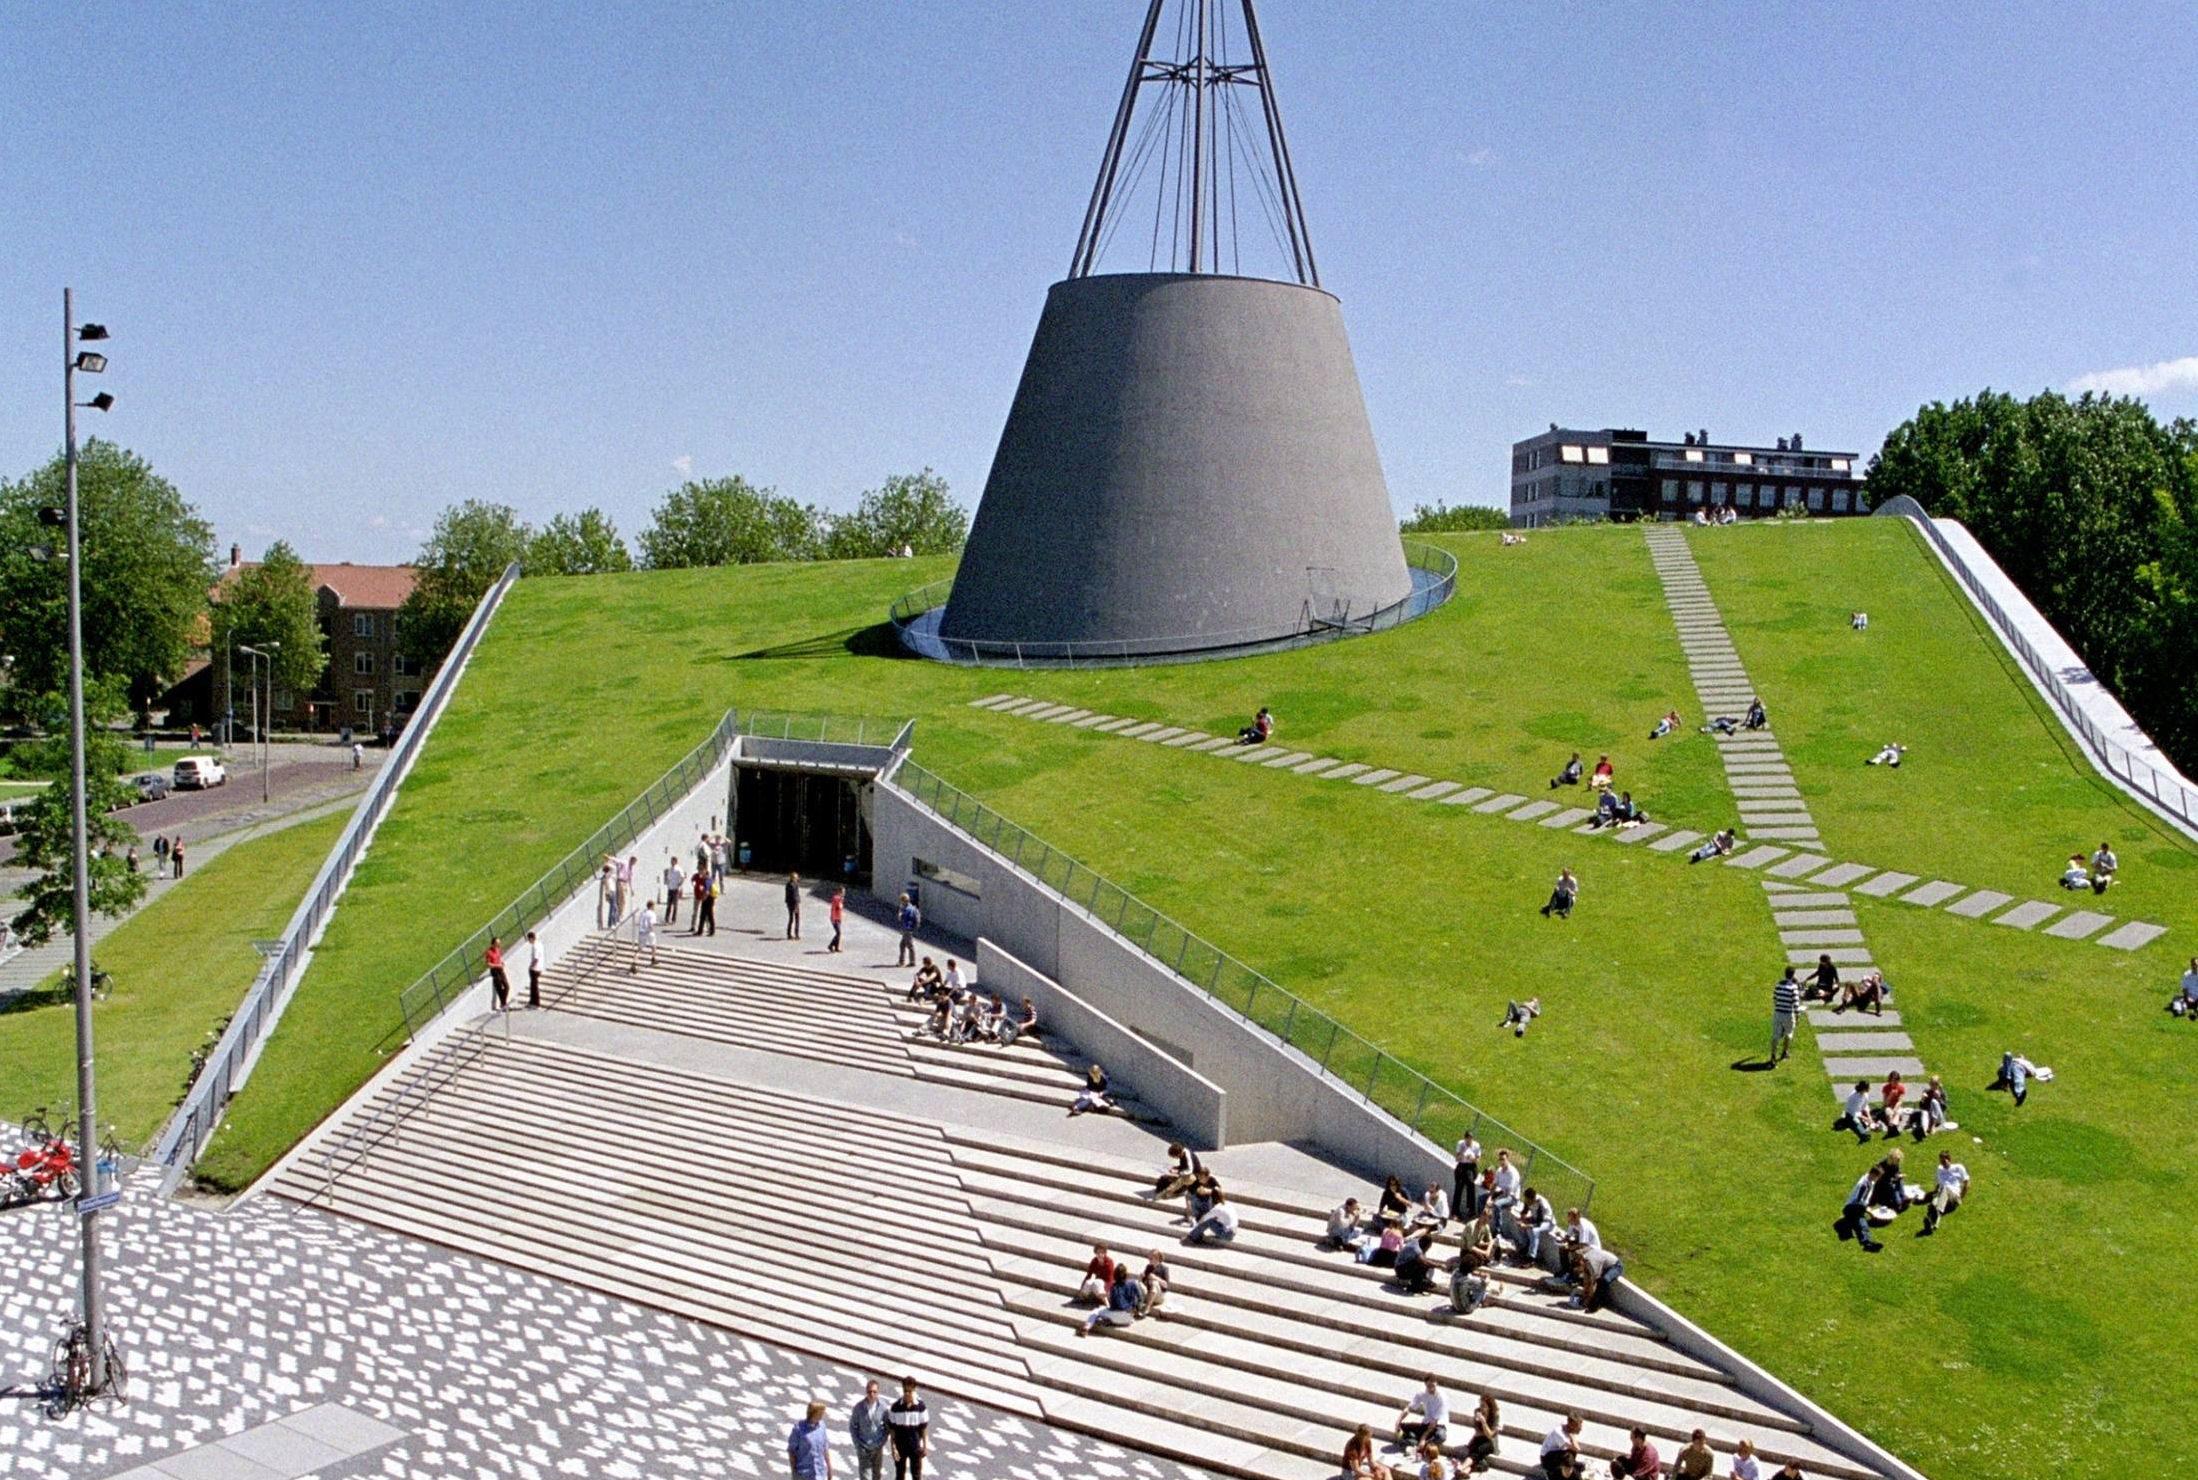
\includegraphics[width=\paperwidth,height=\paperheight]{images/background-titlepage.jpg}}%
\setbeamertemplate{footline}{\usebeamertemplate*{minimal footline}}
\frame{\titlepage}
}


% \section{Fluid Properties}

\section{Euler turbine model }

\begin{frame}
	\frametitle{Euler Turbine model }
	\begin{itemize}
		\item  0-D model for Centripetal Radial Turbine
		\item Solves for each position in the turbine:
		\begin{itemize}
			\item  Total thermodynamic conditions (TC)
			\item  Static thermodynamic conditions (SC)
			\item  Velocity triangle (VT)
		\end{itemize}	
		\item  Three main modelling assumptions:
		\begin{itemize}
			\item  Mass conservation at all turbine states
			\item  Conservation of total enthalpy between stator inlet and outlet
			\item  Conservation of rothalpy between rotor inlet and outlet
		\end{itemize}
		\item  Properties of Toluene included using Coolprop
		\item  Written in Python (including parallized solution domain solving)
	\end{itemize}
\end{frame}


\begin{frame}
	\frametitle{Model schematic }
 	\begin{figure}
 	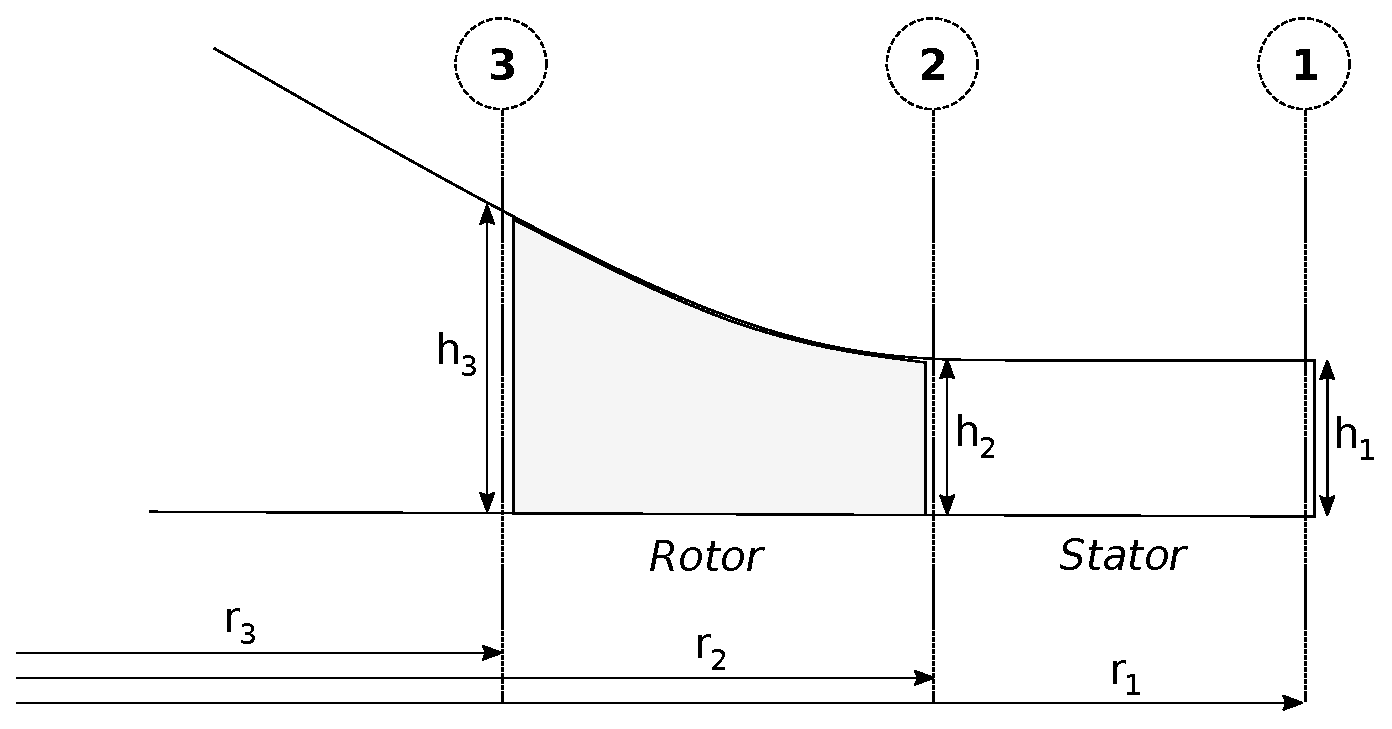
\includegraphics[scale=0.5]{images/eulerturbine.eps}
	 \end{figure}
\end{frame}



\begin{frame}
	\frametitle{Euler Turbine model inputs}
	\begin{tabular}{ll} 
		{\tabitem Radial position and height at each state} & $h_n$, $r_n$ for $n=1,2,3$ \\ \\
		{\tabitem Total conditions at inlet stator and the} & $P_{01}$, $T_{01}$, $||\overline c_1||$, $\alpha_1$ \\ 
		{         direction and magnitude of the velocity} & \\ \\
		{\tabitem Absolute velocity angle at inlet rotor} & $\alpha_2$ \\ \\
		{\tabitem Static pressure at the outlet of the rotor} & $P_3$ \\ \\
		{\tabitem Degree of reaction} & $R$ \\ \\
		{\tabitem Speed of rotation}  & $\omega$ \\ \\
	  \end{tabular}
\end{frame}


\begin{frame}
	\frametitle{Recap important equations }
	\begin{tabular}{ll} 
 		{\tabitem Massflow:} & $\dot{m}=\rho A c_r$ \\ \\ 
       {\tabitem Total Enthalpy:} & $h_0 = h + \frac{||\overline{c}||^2}{2}$ \\ \\
	   {\tabitem Rothalpy:} & $I = h + \frac{||\overline{w}||^2}{2} - \frac{||\overline{U}||^2}{2}$ \\ \\
	   {\tabitem Degree of reaction:} & $R = \frac{h_2-h_3}{h_1-h_3}$ \\ \\
	   {\tabitem Velocity triangles:} & $\overline{c} = \overline{w} + \overline{U}$ \\ \\\
	   {\tabitem Angular velocity:} & $\overline{U}= [U_r, U_\theta]^T = [0 , \omega r]^T$ 
     \end{tabular}
\end{frame}


\begin{frame}
	\frametitle{Model solving procedure }

\begin{enumerate}
	\item Calculate $U_2$ and $U_3$ using $\omega$, $r_2$, and $r_3$
	\item Calculate $TC|_1$, $SC|_1$ and $VT|_1$, using $P_{01}$, $T_{01}$, $||\overline c_1||$ and $\alpha_1$ 
	\item Calculate $m_1$ with $A_3$, $SC|_1$ and $VT|_1$

	\bigskip
	\item Make guess for $||\overline c_2||$
	\item Assuming $h_{01}=h_{02}$, $s_{01}=s_{02}$, calculate $SC|_2$ and $VT|_2$ with $\alpha_2$ and $||\overline c_2||$
	\item Calculate $m_2$ with $SC|_2$, $VT|_2$ and $A_2$
	\item Go back to step 4 until $\dot{m}_1 =\dot{m}_2$
	\bigskip


	\item Calculate $SC|_3$ using $R$, $h_2$, $h_1$ and $P_3$ 
	\item Calculate $c_{r-3}$ with $\dot{m}_1$, $A_3$ and $SC|_3$
	\item Assuming $I_2=I_3$, calculate $||w_3||$ with $h_3$ and $\overline{U}_3$ 
	\item Calculate $VT|_3$ at outlet rotor using $||w_3||$ and $c_{r-3}$
	\item Calculate $TC|_3$ with $VT|_3$ and $SC|_3$ 
\end{enumerate}
\end{frame}



% \begin{frame}
% 	\frametitle{Turbine: Efficiencies and DOR}
% 	\begin{figure}
% 	\includegraphics[scale=0.30]{\resfdir TurbineEffienciesAndDegreeOfReaction.png}
% 	\end{figure}
% \end{frame}

% \begin{frame}
% 	\frametitle{Rotor: Total Enthalpy}
% 	\begin{figure}
% 	\includegraphics[scale=0.30]{\resfdir RotorTotalEnthalpy.png}
% 	\end{figure}
% \end{frame}


%\begin{frame}
%	\frametitle{Stagger Edge Angle: Flowpath Area}
%	\begin{figure}
%	  \begin{subfigure}[b]{0.48\textwidth}
%	    \includegraphics[width=\textwidth]{\resfdir bladeshapeSA.png}
%	    \caption{Bladeshape variation}
%	    \label{fig:1}
%	  \end{subfigure}
%	  \begin{subfigure}[b]{0.48\textwidth}
%	    \includegraphics[width=\textwidth]{\resfdir unfitfpSA.png}
%	    \caption{Flow path}
%	    \label{fig:2}
%	  \end{subfigure}
%	\end{figure}
%\end{frame}
%
%\begin{frame} 
%	\frametitle{Stagger Edge Angle: Fitted height distribution}
%	\begin{figure}
%	  \begin{subfigure}[b]{0.48\textwidth}
%	    \includegraphics[width=\textwidth]{\resfdir fitfpSA.png}
%	    \caption{Fitted flowpath}
%	    \label{fig:1}
%	  \end{subfigure}
%	  \begin{subfigure}[b]{0.48\textwidth}
%	    \includegraphics[width=\textwidth]{\resfdir fithdSA.png}
%	    \caption{Fitted height distribution}
%	    \label{fig:2}
%	  \end{subfigure}
%	\end{figure}
%\end{frame}
%
%
%
%\begin{frame}
%	\frametitle{Leading Edge Angle: Flowpath Area}
%	\begin{figure}
%	  \begin{subfigure}[b]{0.48\textwidth}
%	    \includegraphics[width=\textwidth]{\resfdir bladeshapeLA.png}
%	    \caption{Bladeshape variation}
%	    \label{fig:1}
%	  \end{subfigure}
%	  \begin{subfigure}[b]{0.48\textwidth}
%	    \includegraphics[width=\textwidth]{\resfdir unfitfpLA.png}
%	    \caption{Flow path}
%	    \label{fig:2}
%	  \end{subfigure}
%	\end{figure}
%\end{frame}
%
%\begin{frame}
%	\frametitle{Leading Edge Angle: Fitted height distribution}
%	\begin{figure}
%	  \begin{subfigure}[b]{0.48\textwidth}
%	    \includegraphics[width=\textwidth]{\resfdir fitfpLA.png}
%	    \caption{Fitted flowpath}
%	    \label{fig:1}
%	  \end{subfigure}
%	  \begin{subfigure}[b]{0.48\textwidth}
%	    \includegraphics[width=\textwidth]{\resfdir fithdLA.png}
%	    \caption{Fitted height distribution}
%	    \label{fig:2}
%	  \end{subfigure}
%	\end{figure}
%\end{frame}
%
%
%\begin{frame}
%	\frametitle{Trailing Edge Angle: Flowpath Area}
%	\begin{figure}
%	  \begin{subfigure}[b]{0.48\textwidth}
%	    \includegraphics[width=\textwidth]{\resfdir bladeshapeTA.png}
%	    \caption{Bladeshape variation}
%	    \label{fig:1}
%	  \end{subfigure}
%	  \begin{subfigure}[b]{0.48\textwidth}
%	    \includegraphics[width=\textwidth]{\resfdir unfitfpTA.png}
%	   	\caption{Flow path}
%	    \label{fig:2}
%	  \end{subfigure}
%	\end{figure}
%\end{frame}
%
%\begin{frame}
%	\frametitle{Trailing Edge Angle: Fitted height distribution}
%	\begin{figure}
%	  \begin{subfigure}[b]{0.48\textwidth}
%	    \includegraphics[width=\textwidth]{\resfdir fitfpTA.png}
%	    \caption{Fitted flowpath}
%	    \label{fig:1}
%	  \end{subfigure}
%	  \begin{subfigure}[b]{0.48\textwidth}
%	    \includegraphics[width=\textwidth]{\resfdir fithdTA.png}
%	    \caption{Fitted height distribution}
%	    \label{fig:2}
%	  \end{subfigure}
%	\end{figure}
%\end{frame}
%
%
%
% \begin{frame}
% 	\frametitle{Rotor: Pressure and Mach}
% 	\begin{figure}
% 	  \begin{subfigure}[b]{0.48\textwidth}
% 	    \includegraphics[width=\textwidth]{\resfdir RotorPressure.png}
% 	    \caption{Pressure}
% 	    \label{fig:1}
% 	  \end{subfigure}
% 	  \begin{subfigure}[b]{0.48\textwidth}
% 	    \includegraphics[width=\textwidth]{\resfdir RotorMach.png}
% 	    \caption{Absolute Mach}
% 	    \label{fig:2}
% 	  \end{subfigure}
% 	\end{figure}
% \end{frame}

% \begin{frame}
% 	\frametitle{Rotor: Radial and Tangential Mach}
% 	\begin{figure}
% 	  \begin{subfigure}[b]{0.48\textwidth}
% 	    \includegraphics[width=\textwidth]{\resfdir RotorRMach.png}
% 	    \caption{Absolute Radial Mach}
% 	    \label{fig:1}
% 	  \end{subfigure}
% 	  \begin{subfigure}[b]{0.48\textwidth}
% 	    \includegraphics[width=\textwidth]{\resfdir RotorThetaMach.png}
% 	    \caption{Absolute Tangential Mach}
% 	    \label{fig:2}
% 	  \end{subfigure}
% 	\end{figure}
% \end{frame}

% \begin{frame}
% 	\frametitle{Rotor: Entropy and Temperature}
% 	\begin{figure}
% 	  \begin{subfigure}[b]{0.48\textwidth}
% 	    \includegraphics[width=\textwidth]{\resfdir RotorEntropy.png}
% 	    \caption{Entropy}
% 	    \label{fig:1}
% 	  \end{subfigure}
% 	  \begin{subfigure}[b]{0.48\textwidth}
% 	    \includegraphics[width=\textwidth]{\resfdir RotorTemperature.png}
% 	    \caption{Temperature}
% 	    \label{fig:2}
% 	  \end{subfigure}
% 	\end{figure}
% \end{frame}


% \begin{frame}
% 	\frametitle{Preliminary conclusions }
% 	\begin{itemize}
% 		\item  Increasing rotational speed increases total-to-total efficiency
% 			\begin{itemize}
% 			\item  Less energy is dissipated into heat due to viscosity
% 			\item Seperation bubble becomes much smaller
% 			\end{itemize}
% 		\item  The leading blade angle is more aligned with the flow at higher speeds
% 		\item  Increasing rotational speed past a certain speed ($\approx$ 470 Hz) decreases total-to-static efficiency
% 			\begin{itemize}
% 			\item  More kinetic energy is lost at the outlet of the rotor
% 			\end{itemize}
% 		\item  The difference between de relative outflow angle and the trailing blade angle increases with rotational speed
% 			\begin{itemize}
% 			\item The flow is not sufficiently bend by the blade 
% 			\item Even at low speeds there is a large difference between the relative outflow angle and the trailing angle
% 			\end{itemize}
% 		\end{itemize}
% \end{frame}


% \begin{frame}
% 	\frametitle{Possible routes to take now}
% 	\begin{itemize}
% 		\item  Investigate effect of more blades (Rene's idea)
% 			\begin{itemize}
% 			\item  Hypothesis: More guidance per unit massflow will bend the flow more at higher speeds  $\rightarrow$ reduce kinetic energy losses
% 			\item  Simulations with 47 and 53 blades have been started Friday end of the day, will be done on Monday. 
% 			\end{itemize}

% 		\item  Seperate effects of flow area and number of blades/blade angles
% 			\begin{itemize}
% 				\item changing the number of blades or the blade angles changes the flow area $\rightarrow$ two effects start to play a role
% 				\item script can be developed that changes the height distribution to keep the flow area constant while changing blade angles and number of blades $\rightarrow$ effects can be seperated
% 			\end{itemize}

% 		\item Monday, end of the day, discussion with Quirijn and possibly Jos?

		
% 		\end{itemize}
% \end{frame}

\end{document}
